%%%%%%%%%%%%%%%%%%%%%%%%%%%%%%%%%%%%%%%%%%%%%%%%%%%%%%%%%%%%%%%%%%%%
\section{Data Description}

\subsection{The Role of Descriptive Statistics}

The goal of data analysis is to transform raw data into meaningful information. \textbf{Descriptive Statistics} is the first step, organizing and summarizing data to reveal hidden patterns. Without it, data remains just a meaningless matrix of numbers.

\begin{figure}[H]
    \centering
\includegraphics[scale=0.8]{11.Statistical Learning peapline - Descriptive Statistics.jpg}
    \caption{The role of Descriptive Statistics in the Pipeline}
    \captionsetup{font=footnotesize}
\end{figure}

This stage uses \textbf{Descriptive Statistics} and \textbf{Exploratory Data Analysis (EDA)} to achieve:

\begin{itemize}
    \item \textbf{Data Classification}: Organizing data into categories (e.g., Frequency Tables).
    \item \textbf{Data Summarization}: Calculating core mathematical characteristics:
    \begin{itemize}
        \item \textit{Central Tendency:} Mean, Median, Mode (Where is the center?).
        \item \textit{Dispersion:} Variance, Standard Deviation, Range, IQR (How spread out is it?).
        \item \textit{Shape:} Skewness, Kurtosis (Is it asymmetrical or heavily tailed?).
    \end{itemize}
    \item \textbf{Data Visualization}: Creating charts (Bar, Histogram, Box plot, Scatter, Line) for immediate visual understanding.
    \item \textbf{Outlier Detection \& Hypothesis Checking}: Finding errors and testing initial assumptions.
\end{itemize}

Through \textbf{EDA}, Data Scientists uncover business insights, natural clusters, anomalies, and variable correlations.

%==============================================================================
\subsection{Data Classification}
%==============================================================================

\subsubsection{Unitary vs. Frequency Distributions}

\textbf{1. The Unitary Distribution}\\
The raw sequence of observed values for a variable $X$ across $n$ units (e.g., a raw column in a SQL table):
$$x_1, x_2, \ldots, x_n$$

\textit{Example:} Ages of $n=10$ students: $22, 23, 21, 22, 24, 23, 22, 25, 23, 22$. \\
It contains 100\% of the information but is impossible to read directly when $n$ is large.

\vspace{0.3cm}
\textbf{2. Distinct Modalities ($k$)}\\
The unique, non-repeating values in the dataset: $x_1, \ldots, x_k$.
\begin{itemize}
    \item $n$ = Total observations (rows).
    \item $k$ = Total unique values (categories). Generally, $k \leq n$.
\end{itemize}

\vspace{0.3cm}
\textbf{3. Frequency Distribution Table}\\
Once we identify the $k$ modalities, we count their occurrences.

\begin{itemize}
    \item \textbf{Absolute Frequency ($n_i$)}: Exact count of occurrences. 
    $$\sum_{i=1}^{k} n_i = n$$
    \item \textbf{Relative Frequency ($f_i$)}: Proportion of the total ($f_i = \frac{n_i}{n}$). 
    $$\sum_{i=1}^{k} f_i = 1$$
\end{itemize}

\vspace{0.2cm}
\textit{Example Table (based on the $10$ student ages above):}

\begin{center}
\renewcommand{\arraystretch}{1.2}
\begin{tabular}{|c|c|c|}
    \hline
    \textbf{Modality ($X$)} & \textbf{Abs. Freq. ($n_i$)} & \textbf{Rel. Freq. ($f_i$)} \\
    \hline
    21 & 1 & 0.10 \\
    22 & 4 & 0.40 \\
    23 & 3 & 0.30 \\
    24 & 1 & 0.10 \\
    25 & 1 & 0.10 \\
    \hline
    \textbf{Total} & \textbf{$n=10$} & \textbf{1.00} \\
    \hline
\end{tabular}
\end{center}

\vspace{0.3cm}
\subsubsection{Advantages of Frequency Tables}
\begin{enumerate}
    \item \textbf{Compression}: Shrinks millions of rows ($n$) into a few manageable categories ($k$).
    \item \textbf{Comparability}: Relative frequencies ($f_i$) allow fair comparison between datasets of vastly different sizes.
    \item \textbf{Visualization}: They serve as the exact mathematical blueprint for plotting Bar Charts and Histograms.
\end{enumerate}

\subsection{Data Summarization}

\subsubsection{Statistical Indices}

After creating Frequency Tables, the next step is computing \textbf{Statistical Indices}. These metrics compress the entire dataset into a few key numbers that describe three fundamental aspects:

\begin{enumerate}
    \item \textbf{Central Tendency}: Identifies the \textit{typica} or \textit{center value} of the dataset (Mean, Median, Mode).
    \item \textbf{Variation (Dispersion)}: Measures how spread out the values are from each other (Variance, Standard Deviation, Range, Inter-quartile Range).
    \item \textbf{Shape}: Describes the symmetry and tail behavior of a numerical distribution (Skewness, Kurtosis).
\end{enumerate}

\subsubsection{Special Cases: Zero Variation}

Data summarization is trivial when there is \textbf{no variation} in the dataset:

\begin{itemize}
    \item \textbf{Constant Numerical Variable}: E.g., 100 steel rods all measuring exactly 10.0 mm. The central tendency is 10.0 mm, variation is $0$, and shape is undefined.
    \item \textbf{Single-Category Categorical Variable}: E.g., 50 employees all answering "Yes" to a survey. The mode is "Yes" and there is 100\% homogeneity.
\end{itemize}

In both cases, advanced statistical indices are unnecessary or mathematically undefined. Real-world datasets require summarization precisely because they contain variation.

\subsubsection{Hierarchy of Variable Typology}

The \textbf{scale of measurement} dictates which mathematical operations and statistical methods are valid. Variables follow a strict hierarchy based on their information capacity:

\vspace{0.2cm}
\begin{center}
    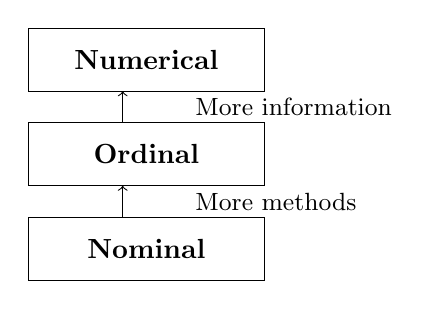
\begin{tikzpicture}
        \node[draw, rectangle, minimum width=3cm, minimum height=0.8cm] at (0,0) {\textbf{Nominal}};
        \node[draw, rectangle, minimum width=3cm, minimum height=0.8cm] at (0,1.2) {\textbf{Ordinal}};
        \node[draw, rectangle, minimum width=3cm, minimum height=0.8cm] at (0,2.4) {\textbf{Numerical}};
        \draw[->] (-0.3,0.4) -- (-0.3,0.8);
        \draw[->] (-0.3,1.6) -- (-0.3,2.0);
        \node[right] at (0.5,1.8) {\small More information};
        \node[right] at (0.5,0.6) {\small More methods};
    \end{tikzpicture}
\end{center}
\vspace{0.2cm}

\textbf{Core Principle:} The higher a variable is in the hierarchy, the more information it carries and the more sophisticated the statistical methods you can apply to it.

\subsubsection{General Rule of Data Processing}

Because of this hierarchy, \textbf{methods designed for lower-level variables work on higher-level variables, but not vice versa}:

\begin{itemize}
    \item \textbf{Nominal methods} (e.g., mode, frequency counts) work on \textit{all} variable types.
    \item \textbf{Ordinal methods} (e.g., median, percentiles, ranking) work on Ordinal and Numerical variables.
    \item \textbf{Numerical methods} (e.g., mean, variance) work \textit{only} on Numerical variables.
\end{itemize}

\vspace{0.2cm}
\begin{center}
\renewcommand{\arraystretch}{1.3}
\begin{tabular}{|l|c|c|c|}
\hline
\textbf{Method Type} & \textbf{Nominal} & \textbf{Ordinal} & \textbf{Numerical} \\
\hline
Nominal methods & \checkmark & \checkmark & \checkmark \\
Ordinal methods & $\times$ & \checkmark & \checkmark \\
Numerical methods & $\times$ & $\times$ & \checkmark \\
\hline
\end{tabular}
\end{center}

\subsection{Measures of Central Tendency}

Measures of central tendency summarize the "\textit{center}" of a data distribution. Based on the variable hierarchy:
\begin{itemize}
    \item \textbf{Mode} can be computed for \textit{Nominal, Ordinal, and Numerical} variables.
    \item \textbf{Median} requires ordered data (\textit{Ordinal and Numerical}).
    \item \textbf{Mean} requires arithmetic operations (\textit{Numerical only}).
\end{itemize}

%==============================================================================
\subsubsection{Mode}

\begin{defbox}{Mode}
The Mode (Mo) is the value of the variable that occurs most frequently in a dataset. 
\end{defbox}

\begin{itemize}
    \item For continuous grouped data, the Mode is estimated as the midpoint of the \textbf{Modal Class} (the interval with the highest frequency density).
    \item A distribution can be unimodal, bimodal, or multimodal.
\end{itemize}

\vs


%==============================================================================
\subsubsection{Median}

\begin{defbox}{Median}
The Median (Me) is the middle value of an ordered distribution ($x_{(1)} \leq x_{(2)} \leq \cdots \leq x_{(n)}$). It divides the data exactly in half (50\% of the observations fall below it, 50\% fall above it).
\end{defbox}

\begin{itemize}
    \item \textbf{Odd $n$}: $\text{Me} = x_{\left(\frac{n+1}{2}\right)}$
    \item \textbf{Even $n$}: $\text{Me} = \frac{x_{\left(\frac{n}{2}\right)} + x_{\left(\frac{n}{2}+1\right)}}{2}$ (for numerical data).
\end{itemize}


%==============================================================================
\subsubsection{Quantiles, Percentiles, and Quartiles}

\begin{defbox}{Quantiles}
A Quantile of order $\alpha$ ($0 < \alpha < 1$) is a value $x_{(l^*)}$ that divides the ordered data such that a proportion $\alpha$ falls below it and $(1-\alpha)$ falls above it:
\begin{equation}
    \frac{l^*}{n} \geq \alpha \quad \text{AND} \quad \frac{l^*-1}{n} < \alpha
\end{equation}
\end{defbox}

\textbf{Key Subdivisions:}
\begin{itemize}
    \item \textbf{Quartiles:} Divide data into 4 parts. $Q_1$ (25th percentile), $Q_2$ (\textbf{Median}, 50th percentile), $Q_3$ (75th percentile). The distance $Q_3 - Q_1$ is the \textit{Interquartile Range (IQR)}.
    \item \textbf{Percentiles:} Divide data into 100 parts ($P_1 \dots P_{99}$).
    \item \textbf{Deciles:} Divide data into 10 parts ($D_1 \dots D_9$).
\end{itemize}

%==============================================================================
\subsubsection{Mean}

\begin{defbox}{Arithmetic Mean ($\mu$)}
The Arithmetic Mean ($\mu$) is the sum of all observed values divided by the total number of units $n$:
\begin{equation}
    \mu = \frac{1}{n} \sum_{l=1}^{n} x_l
\end{equation}
\end{defbox}

If data is in a frequency table with relative frequencies $f_i$: $\mu = \sum_{i=1}^{k} x_i \cdot f_i$ (for grouped continuous data, $x_i$ is the interval midpoint).

\vs
\textbf{Mathematical Property ($L_2$ Minimization - Barycenter):} \\
The Mean minimizes the sum of squared errors (Variance). Because it uses squared distances, it is \textbf{highly sensitive to outliers}.
\begin{equation}
    \min_c \sum_{l=1}^{n} (x_l - c)^2 \quad \text{is achieved when } c = \mu
\end{equation}

\vspace{0.2cm}
\textbf{Fundamental Properties of the Mean:}
\begin{enumerate}
    \item \textbf{Equidistribution (Center of Mass):} $\sum_{l=1}^{n} x_l = n\mu$. This implies that if you were to replace every single observation in your dataset with the mean value $\mu$, the total sum would remain exactly the same. 
    
    \vs
    
    \item \textbf{Linear Transformation (Linearity):} If a new variable $Y$ is created by applying an affine transformation to $X$ (i.e., $Y = a + bX$), the mean of $Y$ undergoes the exact same transformation: $\mu_Y = a + b\mu_X$. This property is fundamental for feature scaling; it allows you to shift (add $a$) or scale (multiply by $b$) variables, such as when converting units or computing standard z-scores—instantly. 
    \vs

    
    \item \textbf{Partition Property (Weighted Mean):} If a dataset is partitioned into $k$ mutually exclusive subgroups, the global mean $\mu$ is simply the weighted average of the individual subgroup means ($\mu_i$). Each subgroup's mean is weighted by its respective size ($n_i$):
    \begin{equation}
        \mu = \frac{1}{n} \sum_{i=1}^{k} \mu_i \cdot n_i
    \end{equation}
    where $n = \sum_{i=1}^{k} n_i$ is the total number of observations. This is highly efficient for aggregating statistics from distributed data chunks or pre-calculated group summaries without needing the original raw data.
\end{enumerate}

%==============================================================================

\subsubsection{Chisini's Definition and Types of Means}

According to the Italian statistician Oscar Chisini, a mean $M$ is not just a single formula, but a generalized concept. It is defined as the single theoretical value that can replace every actual observation in a dataset without altering the overall result of a specific evaluation function $f$:
$$f(x_1, x_2, \dots, x_n) = f(M, M, \dots, M)$$
Depending on the nature of the data and the mathematical operation $f$ we want to preserve, we derive different types of means that are crucial in Data Science:

\begin{itemize}
    \item \textbf{Arithmetic Mean (AM):} Preserves the \textit{Sum} ($f = x_1 + x_2 + \dots + x_n$). It is the default choice for independent, additive data. However, it can be highly misleading when dealing with skewed distributions or multiplicative rates.
    
    \vs

    \item \textbf{Geometric Mean (GM):} Preserves the \textit{Product} ($f = x_1 \cdot x_2 \cdot \dots \cdot x_n$). It is essential when data points compound or act multiplicatively, such as growth rates, financial returns, or when normalizing variables with vastly different scales. 
    $$\text{GM} = \sqrt[n]{\prod_{l=1}^{n} x_l}$$
    
    \item \textbf{Harmonic Mean (HM):} Preserves the \textit{Sum of Reciprocals} ($f = \frac{1}{x_1} + \frac{1}{x_2} + \dots + \frac{1}{x_n}$). It is specifically designed for averaging rates or ratios. In classification tasks, it is the mathematical foundation of the F1-Score: by heavily penalizing extreme low values, it prevents a model with poor precision but perfect recall (or vice versa) from achieving a falsely high average score.
    $$\text{HM} = \frac{n}{\sum_{l=1}^{n} \frac{1}{x_l}}$$
    
    \item \textbf{Quadratic Mean (RMS - Root Mean Square):} Preserves the \textit{Sum of Squares} ($f = x_1^2 + x_2^2 + \dots + x_n^2$). By squaring the values, this mean completely ignores the sign (direction) and disproportionately penalizes larger magnitudes. This makes it the gold standard for evaluating model performance and error magnitudes, such as the Root Mean Square Error (RMSE) in regression pipelines.
    $$M_2 = \sqrt{\frac{1}{n} \sum_{l=1}^{n} x_l^2}$$
\end{itemize}

\textbf{Inequality of Means (for positive values):}
$$RMS \geq AM \geq GM \geq HM$$ 
(Equality holds only if all $x_i$ are identical).

%==============================================================================
\subsubsection{Trimmed Mean}

\begin{defbox}{Trimmed Mean ($\mu_\alpha$)}
The Trimmed Mean ($\mu_\alpha$) is computed by removing a proportion $\alpha/2$ of the smallest observations and $\alpha/2$ of the largest observations from the ordered data, then calculating the arithmetic mean of the remaining $(1-\alpha)$ values.
\end{defbox}

\begin{itemize}
    \item \textbf{Why use it?} It provides a robust measure of central tendency. It ignores extreme outliers (unlike the regular Mean) but still incorporates more data points than the Median.
    \item \textbf{Example:} A 10\% trimmed mean ($\alpha=0.10$) removes the top 5\% and bottom 5\% of the dataset before averaging.
\end{itemize}

\subsection{Measures of Variability}

Measures of variability assess the quality and reliability of central tendency measures by quantifying how spread out the data values are. The choice of measure depends on the variable type:
\begin{itemize}
    \item \textbf{Nominal:} Heterogeneity indices (Gini, Shannon Entropy).
    \item \textbf{Ordinal:} Range, Interquartile Difference.
    \item \textbf{Numerical:} Variance, Standard Deviation, Coefficient of Variation.
\end{itemize}

%==============================================================================
\subsubsection{Heterogeneity Indices (Nominal Variables)}

For categorical variables, variability means how evenly observations are spread across categories. 
\begin{itemize}
  \item \textbf{Perfect Homogeneity} occurs when all units fall into a single category (high reliability of the Mode).

\item \textbf{Perfect Heterogeneity} occurs when units are equally distributed across all $k$ categories (low reliability of the Mode).
\end{itemize}

\pagebreak

\begin{defbox}{Gini Heterogeneity Index}
An index based on squared relative frequencies ($f_i$) that measures how evenly data is distributed across categories.
\begin{equation}
    H = 1 - \sum_{i=1}^{k} f_i^2
\end{equation}

\end{defbox}

Range: $[0, \frac{k-1}{k}]$. Can be normalized by multiplying by $\frac{k}{k-1}$.

\begin{defbox}{Shannon Entropy Index}
An index based on Information Theory that measures the uncertainty or impurity of a categorical distribution.
\begin{equation}
    H' = -\sum_{i=1}^{k} f_i \log f_i
\end{equation}

\end{defbox}

Range: $[0, \log k]$. It is more sensitive to small changes in distribution than Gini.

\vspace{0.2cm}
\begin{example}{Heterogeneity in HDFS System Logs}
Suppose you are analyzing fault detection logs across two different server clusters. You categorize the log status into $k=3$ modalities: Normal, Warning, Error.

\begin{itemize}
    \item \textbf{Cluster A (Stable):} 90\% Normal, 5\% Warning, 5\% Error.
    \item \textbf{Cluster B (Unstable):} 34\% Normal, 33\% Warning, 33\% Error.
\end{itemize}

Let's compute the Gini Index for both:
\begin{itemize}
    \item $H_A = 1 - (0.90^2 + 0.05^2 + 0.05^2) = 1 - (0.81 + 0.0025 + 0.0025) = 1 - 0.815 = 0.185$
    \item $H_B = 1 - (0.34^2 + 0.33^2 + 0.33^2) = 1 - (0.1156 + 0.1089 + 0.1089) \approx 0.666$
\end{itemize}
Cluster A has low heterogeneity (highly concentrated on "Normal"). Cluster B is near perfect heterogeneity (the maximum Gini for $k=3$ is $\frac{2}{3} \approx 0.667$), meaning the system is completely unpredictable.
\end{example}

%==============================================================================
\subsubsection{Positional Measures (Ordinal/Numerical Variables)}

\begin{defbox}{Range}
A basic measure of dispersion that considers only the absolute extreme values of an ordered dataset, calculated as the difference between the maximum and minimum observations. Highly sensitive to outliers.
\begin{equation}
    R = x_{(max)} - x_{(min)}
\end{equation}
\end{defbox}

\begin{defbox}{Interquartile Difference (IQD)}
A robust measure of variability that computes the spread of the central 50\% of the data, calculated as the difference between the third and first quartiles.
\begin{equation}
    IQD = Q_3 - Q_1
\end{equation}
\end{defbox}

%==============================================================================
\subsubsection{Variance, Standard Deviation, and CV (Numerical Variables)}

\begin{defbox}{Deviation}
The numerator of the variance, representing the total sum of squared errors (SSE) from the mean.
\begin{equation}
    Dev(X) = \sum_{l=1}^{n} (x_l - \mu)^2
\end{equation}
\end{defbox}

\begin{defbox}{Variance}
The average squared deviation of each data point from the mean. It quantifies the expected squared error when using the mean as a predictor.
\begin{equation}
    \sigma^2 = \frac{1}{n} \sum_{l=1}^{n} (x_l - \mu)^2
\end{equation}
\end{defbox}

\begin{defbox}{Standard Deviation}
The square root of the variance. It translates the dispersion back into the original unit of measurement, making it directly interpretable.
\begin{equation}
    \sigma = \sqrt{\sigma^2}
\end{equation}
\end{defbox}

\begin{defbox}{Coefficient of Variation (CV)}
A dimensionless, relative measure of variability calculated as the ratio of the standard deviation to the absolute value of the mean.
\begin{equation}
    CV = \frac{\sigma}{|\mu|}
\end{equation}
\end{defbox}

%==============================================================================
\subsubsection{Standardization (Z-Scores)}

\begin{defbox}{Standardization (Z-Score)}
The process of transforming a numerical variable $X$ onto a standard scale by subtracting the mean and dividing by the standard deviation. The resulting variable always has a mean of 0 and a variance of 1.
\begin{equation}
    Z_X = \frac{X - \mu_X}{\sigma_X} \qquad \mu = 0, \quad  \sigma^2=1
\end{equation}
\end{defbox}


The standardized value $Z_X$ represents the number of standard deviations that a particular observation $X$ is away from the mean $\mu_X$:
\begin{itemize}
 \item If $Z_X > 0$: the observation is above the mean.
 \item If $Z_X < 0$: the observation is below the mean.
 \item If $Z_X = 0$: the observation equals the mean.
\end{itemize}

Standardization is particularly useful for:
\begin{enumerate}
 \item Comparing variables measured in different units.
 \item Identifying outliers (typically values with $|Z_X| > 3$).
 \item Computing probabilities in the standard normal distribution.
 \item Preprocessing data for machine learning algorithms.
\end{enumerate}


\vspace{0.2cm}
\begin{example}{\textbf{Engine Telemetry: CV and Standardization}}

You are validating powertrain data and need to compare two sensors with completely different scales:
\begin{itemize}
    \item \textbf{Coolant Temperature ($X_1$):} $\mu = 90^\circ\text{C}$, $\sigma = 5^\circ\text{C}$
    \item \textbf{Injection Pressure ($X_2$):} $\mu = 1800 \text{ bar}$, $\sigma = 300 \text{ bar}$
\end{itemize}

\textbf{1. Comparing Variability (Using CV):} \\
Which sensor is more unstable relative to its baseline? You cannot compare $5^\circ\text{C}$ with $300 \text{ bar}$.
\begin{itemize}
    \item $CV_1 = \frac{5}{90} \approx 0.055$ (5.5\% variation)
    \item $CV_2 = \frac{300}{1800} \approx 0.166$ (16.6\% variation)
\end{itemize}
The injection pressure has much higher relative variability.
\vs

\textbf{2. Detecting Anomalies (Using Z-Scores):} \\
During a test, you register a Temperature spike of $108^\circ\text{C}$ and a Pressure drop to $1050 \text{ bar}$. Which is more anomalous mathematically?
\begin{itemize}
    \item $Z_{\text{Temp}} = \frac{108 - 90}{5} = \frac{18}{5} = +3.6$ 
    \item $Z_{\text{Press}} = \frac{1050 - 1800}{300} = \frac{-750}{300} = -2.5$
\end{itemize}
The temperature spike is $+3.6$ standard deviations above normal (a severe anomaly, typically $|Z| > 3$ is a red flag in fault detection), while the pressure drop is only $-2.5$ standard deviations away. 
\end{example}

%==============================================================================
\subsubsection{Decomposition of Total Deviation (ANOVA principle)}

When dataset $Y$ is divided into $k$ groups based on a categorical variable $X$, the total variability of $Y$ can be decomposed:
\begin{equation}
    Dev(Y) = Dev(B) + Dev(W)
\end{equation}

\begin{itemize}
    \item \textbf{Between-Group Deviation ($Dev(B)$):} Measures how much the group means differ from the overall mean. Represents the variance \textit{explained} by the grouping variable $X$.
    \item \textbf{Within-Group Deviation ($Dev(W)$):} Measures how much observations vary around their specific group mean. Represents the variance \textit{unexplained} by $X$ (noise).
\end{itemize}

The \textbf{Correlation Ratio ($\eta^2$)} measures the proportion of variance explained by the groups:
\begin{equation}
    \eta^2 = \frac{Dev(B)}{Dev(Y)}
\end{equation}

\subsection{Shape of Unitary Distribution}

The shape of a quantitative variable's distribution is fundamental for selecting the right statistical models and identifying anomalies. It is defined by four main properties:

\begin{enumerate}
    \item \textbf{Symmetry}: Whether the left and right sides mirror each other.
    \item \textbf{Modality (Peaks)}: The number of distinct peaks (modes).
    \item \textbf{Skewness}: The direction and degree of asymmetry.
    \item \textbf{Kurtosis}: The heaviness of the tails (presence of extreme outliers).
\end{enumerate}

%==============================================================================
\subsubsection{Symmetry and Modality}

\begin{defbox}{Symmetry}
A distribution is perfectly symmetric when its left and right sides are mirror images around the center. In this ideal scenario:
\begin{equation}
    \text{Mean} = \text{Median} = \text{Mode}
\end{equation}
\end{defbox}

\begin{figure}[H] 
    \centering
\includegraphics[scale=0.4]{51.Symmetrical Distribution.jpeg}
    \caption{Symmetrical Distribution}\captionsetup{font=footnotesize}
\end{figure}

\begin{defbox}{Modality (Number of Peaks)}
Describes the number of local maxima in the distribution:
\begin{itemize}
    \item \textbf{Unimodal}: One clear peak (e.g., standard Bell-curve).
    \item \textbf{Bimodal / Multimodal}: Two or more peaks. In Data Science, this is a strong indicator that your dataset contains mixed populations or distinct subgroups that should probably be clustered or separated.
\end{itemize}
\end{defbox}

%==============================================================================
\subsubsection{Skewness}

\begin{defbox}{Skewness}
Measures the degree and direction of asymmetry.
\begin{itemize}
    \item \textbf{Positive (Right) Skewness}: Tail extends to the right. Driven by rare high values. (\textit{Mean $>$ Median $>$ Mode}).
    \item \textbf{Negative (Left) Skewness}: Tail extends to the left. Driven by rare low values. (\textit{Mean $<$ Median $<$ Mode}).
\end{itemize}
\end{defbox}

\begin{figure}[H] 
    \centering
\includegraphics[scale=0.45]{15.Skewness.jpeg}
    \caption{Skewness}\captionsetup{font=footnotesize}
\end{figure}

To quantify skewness, we use different coefficients depending on our need for robustness against outliers:

\begin{enumerate}
    \item \textbf{Pearson's Coefficient (Moment-based):}
    \begin{equation}
        \text{Skewness}_{\text{Pearson}} = \frac{3(\text{Mean} - \text{Median})}{\text{Standard Deviation}}
    \end{equation}
    \textit{Pros/Cons:} Standard metric, but highly sensitive to extreme outliers because it relies on the Mean and Standard Deviation.

    \item \textbf{Bowley's Coefficient (Quartile-based):}
    \begin{equation}
        \text{Skewness}_{\text{Bowley}} = \frac{Q_3 + Q_1 - 2Q_2}{Q_3 - Q_1}
    \end{equation}
    \textit{Pros/Cons:} Highly robust to outliers because it only uses the central 50\% of the data ($Q_1, Q_2, Q_3$). Range is $[-1, 1]$.

    \vs
    \item \textbf{Kelly's Coefficient (Decile-based):}
    \begin{equation}
        \text{Skewness}_{\text{Kelly}} = \frac{P_{90} + P_{10} - 2P_{50}}{P_{90} - P_{10}}
    \end{equation}
    \textit{Pros/Cons:} A great compromise. Uses 80\% of the data, making it more informative than Bowley but more robust than Pearson.
\end{enumerate}

%==============================================================================
\subsubsection{Kurtosis}

\begin{defbox}{Kurtosis}
Measures the \textit{tailedness} of a distribution compared to a standard Normal Distribution ($k=0$). It indicates the propensity of the data to produce extreme outliers.
\end{defbox}

\begin{itemize}
    \item \textbf{Leptokurtic ($k > 0$):} Heavy tails and a sharp peak. High probability of extreme values/outliers. \textit{Data Science Action:} Investigate outliers immediately; consider using robust ML models (like Tree-based models) rather than linear ones.
    \item \textbf{Mesokurtic ($k = 0$):} Normal distribution behavior.
    \item \textbf{Platykurtic ($k < 0$):} Light tails and a flat peak. Extreme outliers are rare. Often implies the data is artificially bounded or truncated.
\end{itemize}

\begin{figure}[H] 
    \centering
\includegraphics[scale=0.35]{16.Kurtosis.jpeg}
    \caption{Kurtosis: sharpness of a distribution}\captionsetup{font=footnotesize}
\end{figure}

%==============================================================================
\vspace{0.3cm}
\begin{example}{\textbf{The Impact of Outliers on Shape Metrics}}

Consider the salary data (in thousands) of a 10-person startup:
$$X = \{25, 28, 30, 32, 35, 38, 42, 48, 55, 120\}$$

The value $120$ (perhaps the CEO's salary) is a massive outlier. Let's see how it affects our shape metrics.

\textbf{1. Basic Statistics:}
\begin{itemize}
    \item Mean ($\mu$) = $45.3$
    \item Median ($Q_2$) = $36.5$
    \item Standard Deviation ($\sigma$) = $27.84$
\end{itemize}
Since Mean $>$ Median, we know the distribution is Right-Skewed.

\textbf{2. Measuring Skewness (Pearson vs. Bowley):}
\begin{itemize}
    \item \textbf{Pearson:} 
    $$ \text{Skew}_{P} = \frac{3(45.3 - 36.5)}{27.84} = +0.948 $$
    The Pearson metric shows an extremely strong right skew, almost entirely driven by the distance between the CEO's salary and the rest of the team.
    
    \item \textbf{Bowley:} We need the quartiles. $Q_1 \approx 29$, $Q_2 = 36.5$, $Q_3 \approx 45$.
    $$ \text{Skew}_{B} = \frac{45 + 29 - 2(36.5)}{45 - 29} = \frac{1}{16} = +0.0625 $$
    Bowley's metric shows a very slight right skew ($+0.06$).
\end{itemize}

\textbf{Conclusion for a Data Scientist:}
Pearson tells you "the whole dataset is heavily skewed." Bowley tells you "the core 50\% of the employees have a fairly symmetric salary distribution." Both are mathematically correct, but Bowley prevents the single outlier from masking the true behavior of the majority of your data. This dataset would also exhibit high \textbf{Leptokurtic} behavior due to that massive right tail.
\end{example}
